%!TEX root = ../../novoIndex.tex

\emph{Machine Learning} (ML), também chamado de Aprendizado de Máquina, é uma subárea da Inteligência Artificial que trata do estudo sistemático de algoritmos e sistemas que são capazes de melhorar seu desempenho com a experiência. Um algoritmo neste domínio é capaz de aprender a partir de dados, capturando padrões e efetuando inferências. Estes algoritmos podem ser entendidos em uma analogia com  humanos e outros animais que, ao se depararem com determinada situação, costumam procurar lembranças de situações similares, de como agiram, e se o comportamento adotado foi vantajoso, e deve ser repetido, ou prejudicial, devendo ser evitado \cite{marsland2015machine,goodfellow2016deep,flach2012machine}.

Para consolidar o aprendizado, os algoritmos de ML precisam passar por um processo de aquisição da experiência, comumente chamado de treinamento. De acordo Mitchell \cite{mitchell1997machine}, um algoritmo que aprende a partir da experiência $E$ quanto a um conjunto de tarefas $T$ e medida de performance $P$, se sua performance nas tarefas em $T$, medida por $P$, melhora com a experiência $E$.

\begin{sidewaysfigure}
	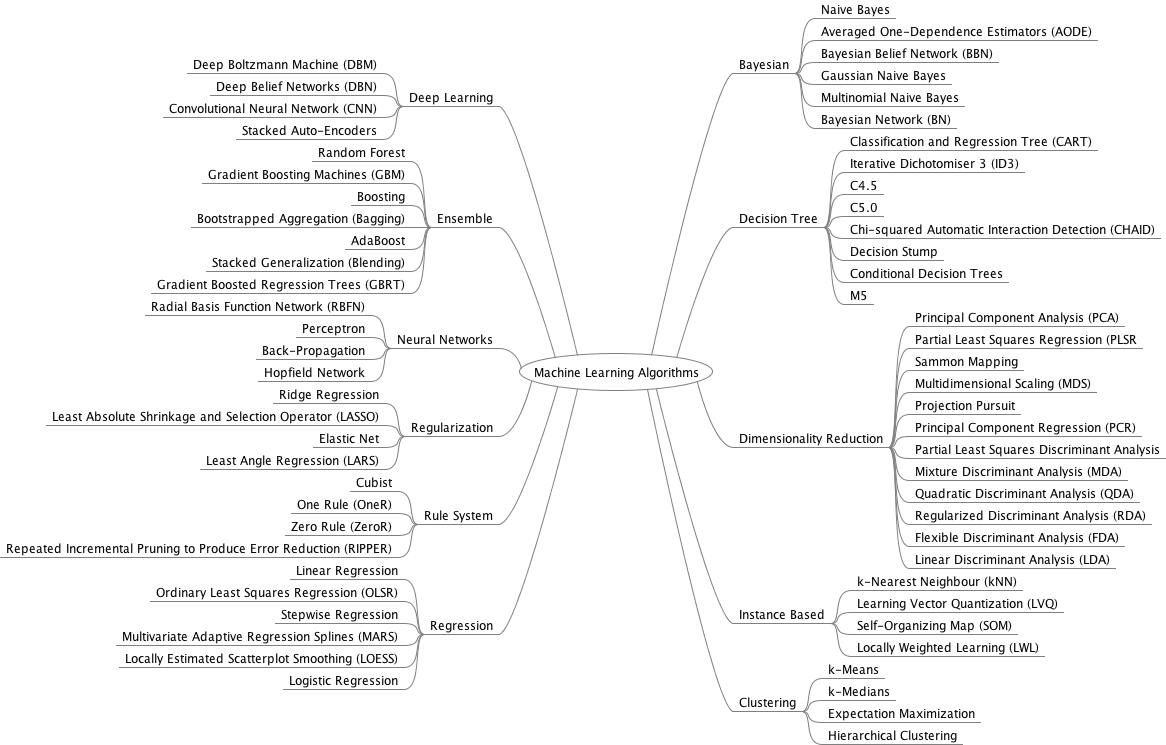
\includegraphics[width=\linewidth]{img/machinelearningalgorithms.png}
	\caption{Mapa mental dos algoritmos de \emph{Machine Learning} organizados por área e sub-área \cite{ml:algos}.}\label{fig:ml_algorithms}
\end{sidewaysfigure}

Ao preparar um algoritmo de ML para desenvolver determinada tarefa, busca-se um modelo, ou seja, uma função, que mapeie as instâncias do espaço de entrada para o de saída \cite{flach2012machine}. Estes modelos podem ser agrupados em diferentes categorias ao se considerar o tipo de aprendizado e a saída desejada para o algoritmo. A Figura \ref{fig:ml_algorithms} apresenta uma visão geral do estado da arte acerca dos modelos de ML e suas subdivisões.

Quanto ao tipo de aprendizado, as tarefas de ML podem ser agrupadas em três tipos diferentes, a depender da presença e do tipo de resposta dada ao algoritmo quanto ao desempenho de suas saídas. No \emph{aprendizado supervisionado}, o algoritmo deve aprender a inferir valores a partir de atributos preditores e do respectivo atributo alvo fornecido como exemplo, ou seja, de cenários em que os valores de saída são conhecidos. Os modelos mais frequentemente utilizados neste tipo de aprendizado são as máquinas de vetores de suporte, redes neurais artificiais \emph{feedforward}, regressão linear e logística, etc. Já no \emph{aprendizado não-supervisionado}, o algoritmo deve inferir padrões e estruturas a partir de dados não rotulados, buscando alguma estrutura interna que os caracterize. Exemplos de modelos aplicáveis a este cenário são os algoritmos \emph{k-means} e \emph{k-medoids}.  Por fim, no \emph{aprendizado por reforço} o algoritmo não recebe dados nem tampouco rótulos, e deve aprender a partir das recompensas positivas ou negativas dadas por ações que modifiquem o ambiente de maneira satisfatória ou não \cite{flach2012machine}.

Quanto ao tipo de saída desejada, os problemas que podem ser endereçados segundo ML são de classificação, regressão, transcrição, tradução automática, detecção de anomalia, síntese e amostragem. No caso do aprendizado supervisionado, em particular, as principais tarefas realizadas são de classificação e regressão \cite{flach2012machine}.

Um algoritmo proposto a uma tarefa de classificação deve especificar cada entrada $x$ como pertencente a uma dentre $k$ categoritas pré-determinadas, produzindo uma saída $y=f(x)$ tal que a função $f$ é definida como $f: \mathds{R}^n \rightarrow \{1, \ldots, k\}$, ou seja, $f$ mapeia sequências de números reais  $x$ de dimensão $n$ para um valor inteiro $y$ dentre $k$ possibilidades \cite{goodfellow2016deep}. Dentre as tarefas de classificação estão, por exemplo, o reconhecimento de objetos em uma imagem, determinar se um indivíduo será ou não vítima de determinada doença, se sobreviverá ou não a determinado acidente, etc.

Numa tarefa de regressão, por sua vez, objetiva-se aprender uma função de valor real a partir de uma entrada \cite{flach2012machine}. Assim, a saída $y=f(x)$ é dada pela função $f: \mathds{R}^n \rightarrow \mathds{R}$, ou seja, $f$ mapeia uma entrada multidimensional $x$ para um valor $y$ real \cite{goodfellow2016deep}. Algumas tarefas de regressão envolvem a previsão de preços de um mercado de ações, a determinação do risco do seguro para um carro, do volume diário de precipitação em determinada cidade, entre outros.

Os modelos de ML são organizados em dois grandes grupos, dos tipos paramétricos ou não paramétricos. Segundo Russel e Norvig, um modelo de aprendizado que resume dados utilizando um conjunto de parâmetros de tamanho definidos independente do número de exemplos de treinamento é chamado de \emph{modelo paramétrico}. Dentre os modelos paramétricos está a regressão logística. Já um \emph{modelo não-paramétrico} é aquele que não pode ser caracterizado por um conjunto limitado de parâmetros. Alguns exemplos de modelos não-paramétricos são máquinas de vetores de suporte, redes neurais artificiais, $k$ vizinhos mais próximos e árvores de decisão CART e C4.5 \cite{russell2016artificial}.

Dentre os modelos não paramétricos, as redes neurais artificiais têm demonstrado resultados satisfatórios em tarefas de classificação e regressão quando aplicadas em diversas áreas. Em especial, aplicações de \emph{Deep Learning} no reconhecimento de objetos e no processamento de linguagem natural, por exemplo, têm trazido ainda mais atenção a este modelo. Diante desta importância e da utilização no contexto deste trabalho, estes conceitos serão abordados com mais profundidade nas seções a seguir.
